% Graphical methodology – Jicoteas por pipá
% 3 x 3 cajas en zig-zag

\documentclass[border=1cm]{standalone}
\usepackage[utf8]{inputenc}
\usepackage{tikz}
\usetikzlibrary{positioning, arrows.meta}
\usetikzlibrary{shapes.geometric, arrows.meta, positioning}

% Estilos de la plantilla (cajas de colores)
\tikzstyle{startstop} = [
  rectangle, rounded corners,
  minimum width=4cm, minimum height=1.6cm,
  text centered, align=center,
  draw=black, fill=red!30
]

\tikzstyle{process} = [
  rectangle,
  minimum width=4cm, minimum height=1.6cm,
  text centered, align=center,
  draw=black, fill=orange!30
]

\tikzstyle{data} = [
  trapezium,
  trapezium left angle=70, trapezium right angle=110,
  minimum width=4cm, minimum height=1.6cm,
  text centered, align=center,
  draw=black, fill=blue!25
]

\tikzset{
  arrow/.style={- {Stealth[length=4mm,width=3mm]}, very thick}
}

\tikzset{
  arrow/.style={
    very thick,
    -{Stealth[length=5mm,width=3mm]}
  }
}


\begin{document}

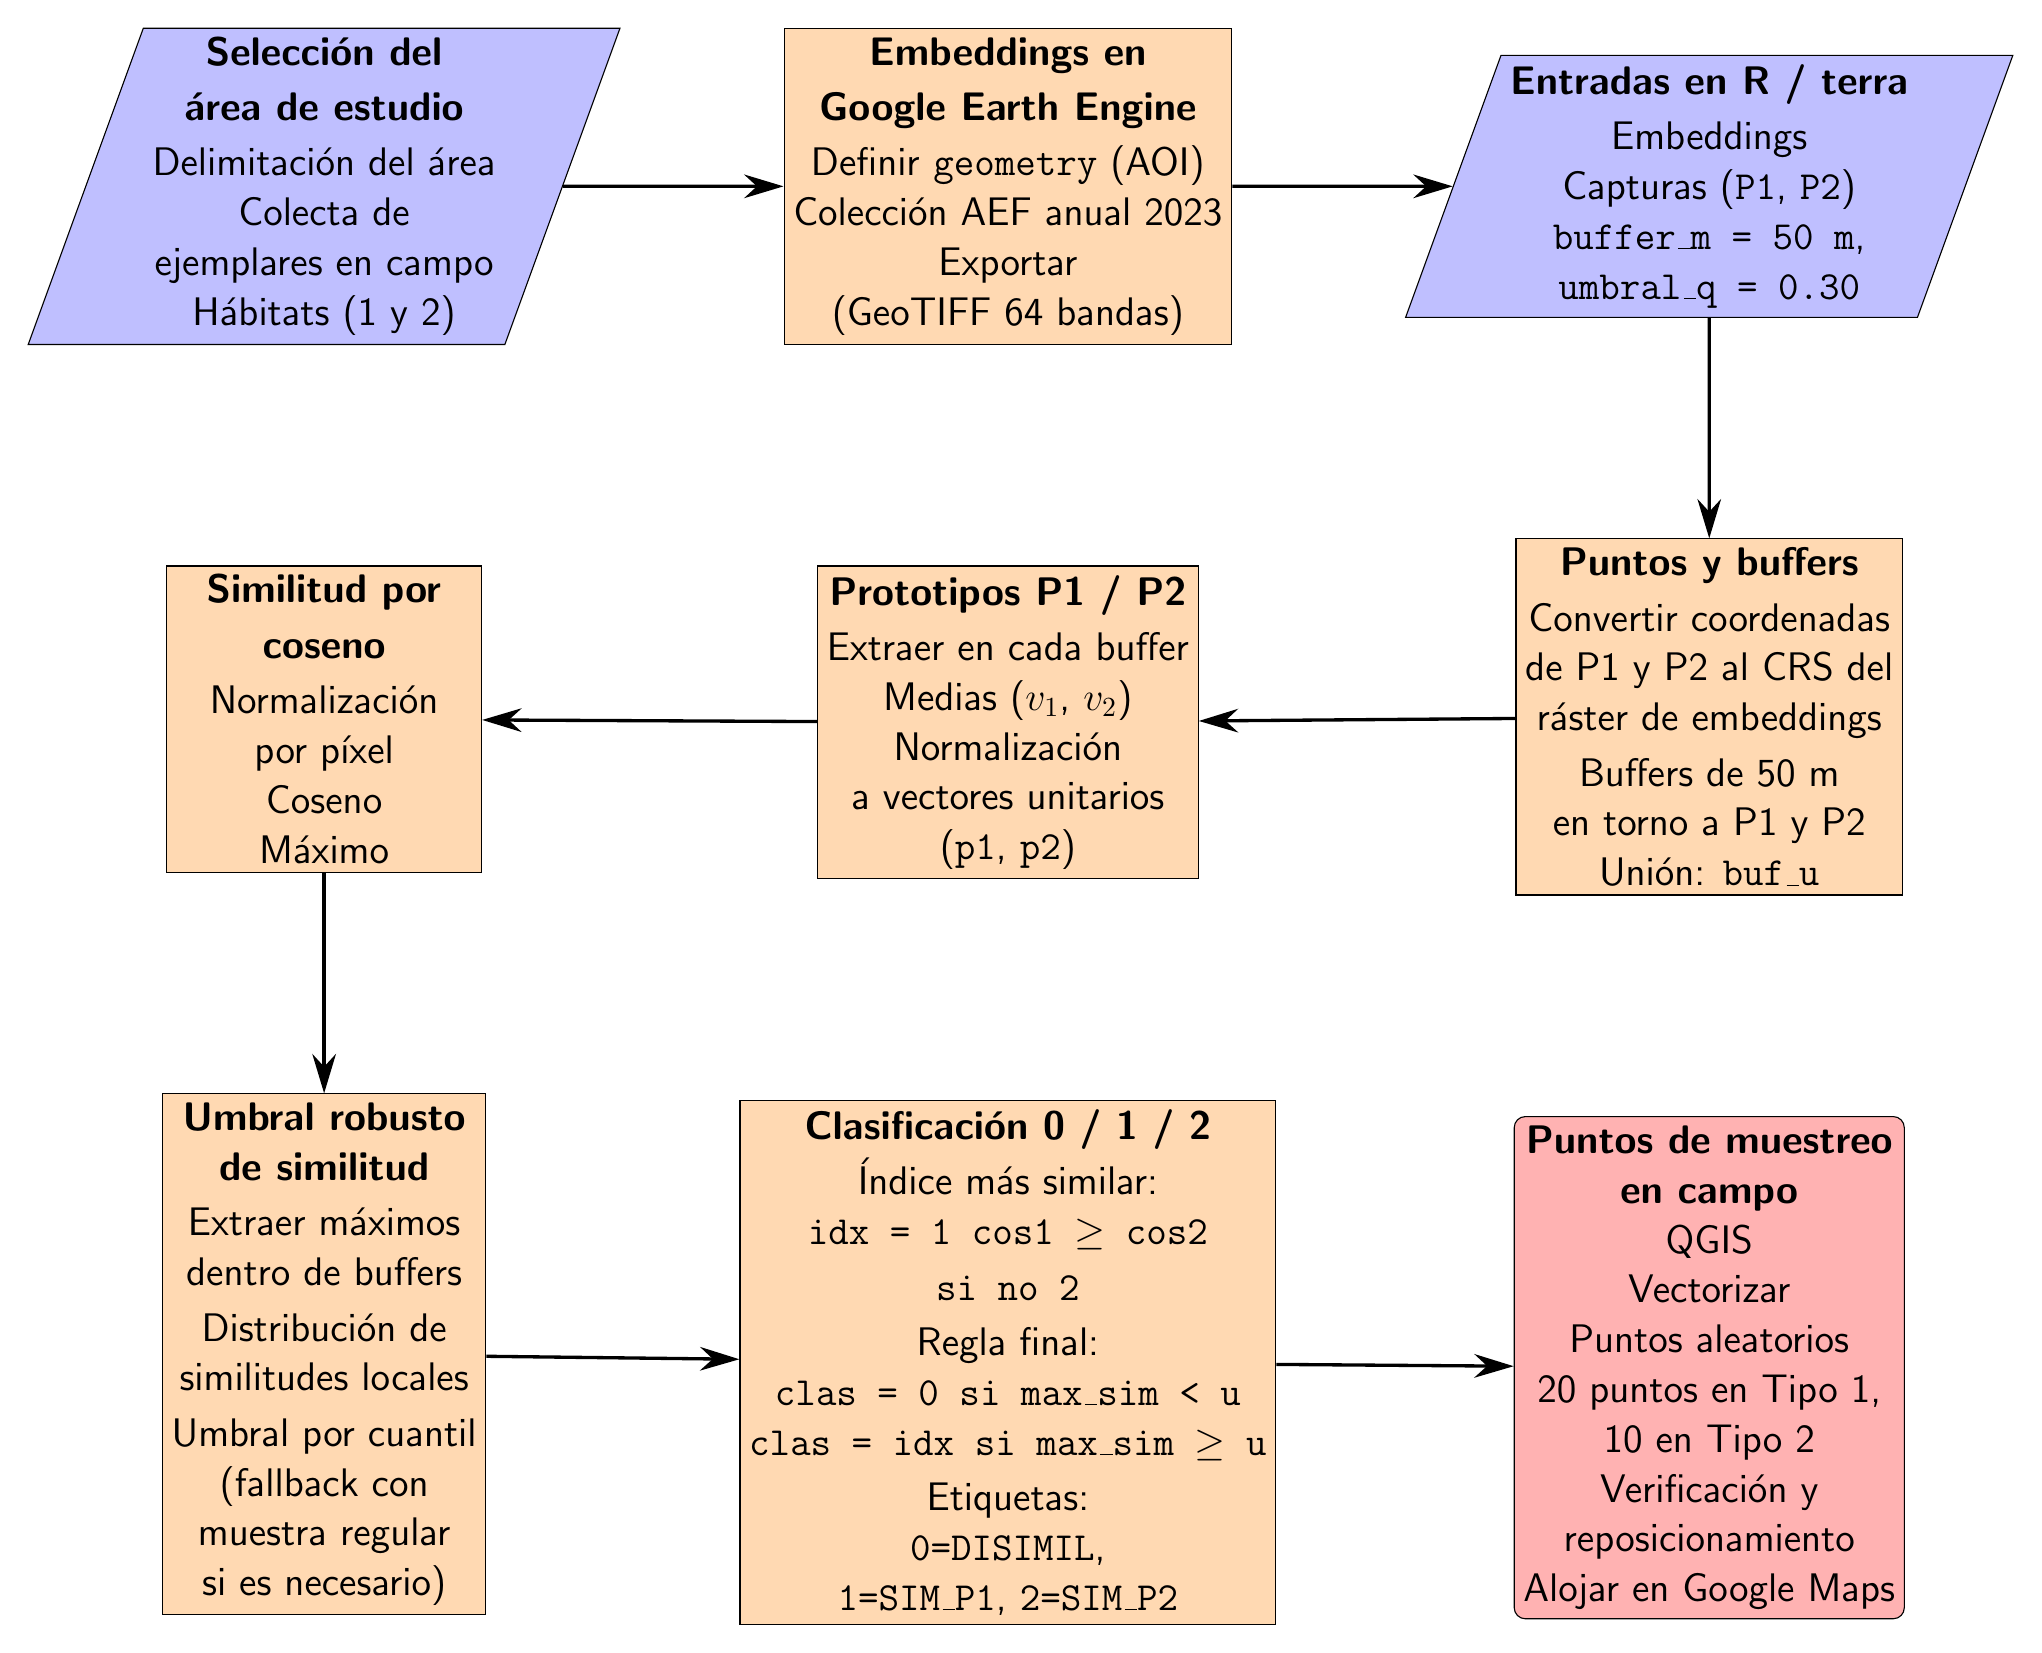
\begin{tikzpicture}[
  font=\sffamily\Large,
  node distance=2.8cm and 2.8cm
]

% ------------------------------------------------
% FILA 1 (arriba): 3 cajas
% ------------------------------------------------

% n1: Selección de área + campo
\node[data] (n1) {%
  \textbf{Selección del}\\[2pt]
  \textbf{área de estudio}\\[2pt]
  Delimitación del área\\
  Colecta de \\
  ejemplares en campo\\
  Hábitats (1 y 2)
};

% n2: Trabajo en GEE
\node[process, right=of n1] (n2) {%
  \textbf{Embeddings en}\\[2pt]
  \textbf{Google Earth Engine}\\[2pt]
  Definir \texttt{geometry} (AOI)\\
  Colección AEF anual 2023\\
  Exportar\\
  (GeoTIFF 64 bandas)
};

% n3: Entradas en R
\node[data, right=of n2] (n3) {%
  \textbf{Entradas en R / terra}\\[2pt]
  Embeddings\\
  Capturas (\texttt{P1}, \texttt{P2})\\
  \texttt{buffer\_m = 50 m},\\
  \texttt{umbral\_q = 0.30}
};

% ------------------------------------------------
% FILA 2 (medio): 3 cajas
% ------------------------------------------------

% n4: Puntos y buffers (debajo de n3 para seguir zig-zag)
\node[process, below=of n3] (n4) {%
  \textbf{Puntos y buffers}\\[2pt]
  Convertir coordenadas \\
  de P1 y P2 al CRS del \\
  ráster de embeddings\\[2pt]
  Buffers de 50 m \\
  en torno a P1 y P2\\
  Unión: \texttt{buf\_u}
};

% n5: Prototipos (a la izquierda de n4)
\node[process, below=of n2] (n5) {%
  \textbf{Prototipos P1 / P2}\\[2pt]
  Extraer en cada buffer\\
  Medias ($v_1$, $v_2$)\\
  Normalización \\
  a vectores unitarios\\
  (\texttt{p1}, \texttt{p2})
};

% n6: Similitud por coseno (a la izquierda de n5)
\node[process, below=of n1] (n6) {%
  \textbf{Similitud por}\\[2pt]
  \textbf{coseno}\\[2pt]
  Normalización \\
  por píxel\\
  Coseno\\
  Máximo
};

% ------------------------------------------------
% FILA 3 (abajo): 3 cajas
% ------------------------------------------------

% n7: Umbral robusto (debajo de n6)
\node[process, below=of n6] (n7) {%
  \textbf{Umbral robusto}\\
  \textbf{de similitud}\\[2pt]
  Extraer máximos \\
  dentro de buffers\\[2pt]
  Distribución de \\
  similitudes locales\\[2pt]
  Umbral por cuantil\\
  (fallback con\\
  muestra regular\\
  si es necesario)
%  \textbf{Umbral robusto}\\
%  \textbf{de similitud}\\[6pt]  
%  Extraer máximos \\
%  en buffers\\
%  Similitudes locales\\[2pt]
%  Umbral y fallback
};

% n8: Clasificación 0/1/2 (a la derecha de n7)
\node[process, below=of n5] (n8) {%
  \textbf{Clasificación 0 / 1 / 2}\\[2pt]
  Índice más similar:\\
  \texttt{idx = 1 cos1 $\ge$ cos2}\\[2pt]
  \texttt{si no 2}\\[2pt]  
  Regla final:\\
  \texttt{clas = 0 si max\_sim < u}\\
  \texttt{clas = idx si max\_sim $\ge$ u}\\[2pt]
  Etiquetas: \\
  \texttt{0=DISIMIL},\\
  \texttt{1=SIM\_P1}, \texttt{2=SIM\_P2}
};

% n9: Puntos aleatorios + Google Maps (a la derecha de n8)
\node[startstop, below=of n4] (n9) {%
  \textbf{Puntos de muestreo}\\
  \textbf{en campo}\\
  QGIS \\
  Vectorizar\\
  Puntos aleatorios\\
  20 puntos en Tipo 1,\\
  10 en Tipo 2\\
  Verificación y\\
  reposicionamiento\\
  Alojar en Google Maps
};

% ------------------------------------------------
% FLECHAS EN ZIG-ZAG (1→2→3→4→5→6→7→8→9)
% ------------------------------------------------

% Fila 1 (izquierda a derecha)
\draw[arrow] (n1) -- (n2);
\draw[arrow] (n2) -- (n3);

% De n3 (arriba derecha) a n4 (medio derecha)
\draw[arrow] (n3) -- (n4);

% Fila 2 (derecha a izquierda)
\draw[arrow] (n4) -- (n5);
\draw[arrow] (n5) -- (n6);

% De n6 (medio izquierda) a n7 (abajo izquierda)
\draw[arrow] (n6) -- (n7);

% Fila 3 (izquierda a derecha)
\draw[arrow] (n7) -- (n8);
\draw[arrow] (n8) -- (n9);

\end{tikzpicture}

\end{document}
